\section{Sensor}
Sensoren som bliver beskrevet i hardware afsnittet skal kommunikere med arduino boardet. Dette kræver nogle trin som kan findes i databladet til sensoren. På figur \ref{sensor_kom} ses et overblik over funktioner gruppen har lavet, som skal til for at aflæse sensoren. Disse funktioner er konstrueret ved at anvende databladet hvor det ses at tre trin skal følges til punkt og prikke for at kunne tilgå sensoren. De tre trin er en initialization, ROM command of function command.
\\
\\
I databladet ses et flowchart over de forskellige veje sensoren kan tilgåes og funktioner den kan udføere. Ud fra dette flowchart har gruppen konstrueret en mindre version, som indeholde de minimums funktioner der skal anvendes for at kunne tilgå sensoren og aflæse denne. Dette ses på figur \ref{sensor_kom}.

\begin{figure}[h!]
  \centering
  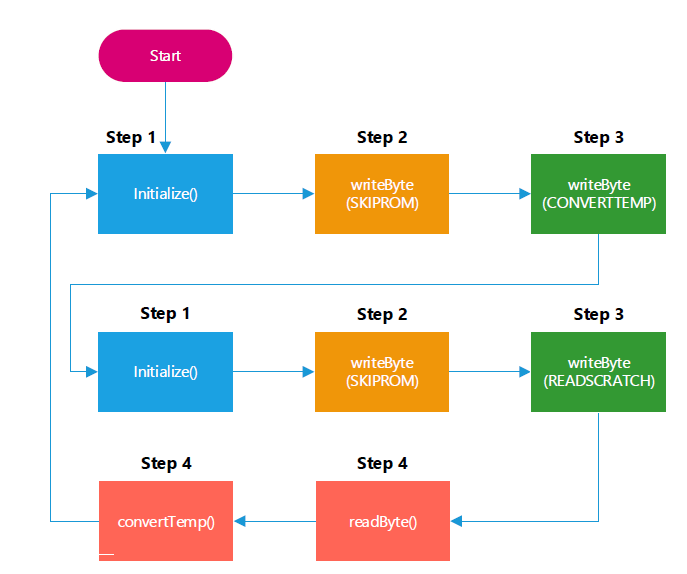
\includegraphics[width=0.8\textwidth]{figures/sensor_communication.png}
  \caption{Kommunikation med sensor.}
  \label{sensor_kom}
\end{figure}
\fxnote{ret størrelse til på alle billeder(noget der skal gøres til sidst!)}

Navne som ses på figur \ref{sensor_kom} er de funktions navne som er givet i vores software. De følger flowchartet for det mindste der skal til for at tilgå og aflæse en temperatur måling af sensoren. Måden de er konstureret på vil blive forklaret i følgende underafsnit.


\subsection{Initialize()}
Initialiserings funktionen som ses på figur \ref{sensor_kom} er konstrueret ved at finde de timings der skal til for at kunne tilgå sensoren over en 1-wire forbindelse. Disse er aflæst af en graf fra databladet (jf. figur \ref{sensor_kom}).




\begin{figure}[h!]
  \centering
  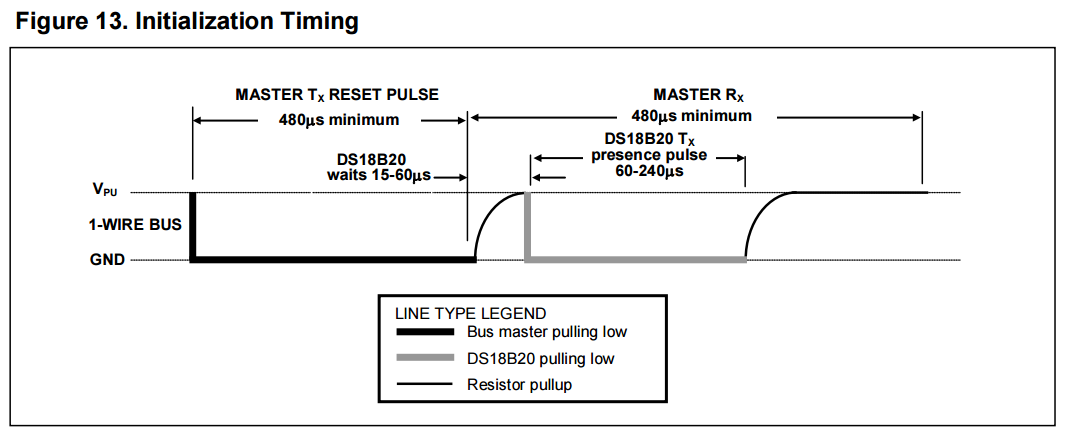
\includegraphics[width=0.5\textwidth]{figures/Initialization_timing.png}
  \caption{Fra datablad om hvordan sensor skal initialiseres.}
  \label{sensor_kom}
\end{figure}

Fra databladet ses det at 1-wire forbindelsen skal have en reset pulse i minimum 480$\mu$S og en presence pulse i 60 til 240$\mu$S. Dette gøres ved at sende et low signal som reset pulse og derefter sætte forbindelsen i tri-state og pull-up modstanden vil trække signalet højt. 
\\
\\
I koden gøres dette ved at bruge digitalWrite til low i kombination med et delay på 500$\mu$S. Derefter sættes pinMode til input og et delay på 500$\mu$S anvendes igen. Dette kan ses på figur \ref{sensor_kode}.

\begin{figure}[h!]
  \centering
  \includegraphics[width=1\textwidth]{figures/Init.png}
  \caption{Initialisering kode.}
  \label{sensor_kode}
\end{figure}

\fxnote{evt noget afslutning på dette underafsnit?}

\subsection{writeByte()}
WriteByte() er en funktion som er blevet konstrueret på samme fremgangsmåde som Initialize() funktionen ved at aflæse en graf der indeholde timings der skal til for at tilgå sensoren.

\begin{figure}[h!]
  \centering
  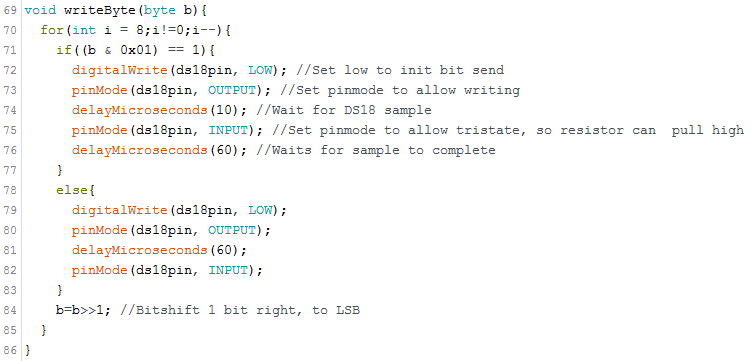
\includegraphics[width=1\textwidth]{figures/write_byte.png}
  \caption{writeByte() arduino kode.}
  \label{write_byte}
\end{figure}
\fxnote{set firkant eller noget rundt om alle vores kodeeksempler så de ikke går i et med teksten omkring}

writeByte 